\item A smooth horizontal disc rotates with a constant angular velocity $\omega$ about a stationary vertical axis passing through its centre, the point $O$. At a moment $t = 0$ a disc is set in motion from that point with velocity $v_0$. Find the angular momentum $M(t)$ of the disc relative to the point $O$ in the reference frame fixed to the disc. Make sure that this angular momentum is caused by the Coriolis force.
    \begin{center}
        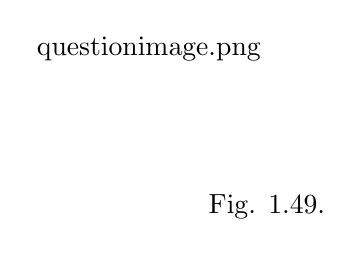
\begin{tikzpicture}
            \node at (0,0) {{questionimage.png}};
            \node at (1.5,-2) {Fig. 1.49.};
        \end{tikzpicture}
    \end{center}
    \begin{center}
        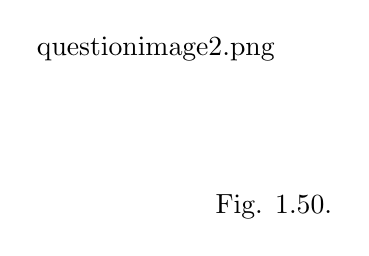
\begin{tikzpicture}
            \node at (0,0) {{questionimage2.png}};
            \node at (1.5,-2) {Fig. 1.50.};
        \end{tikzpicture}
    \end{center}\begin{solution}
    \begin{center}
        \begin{tikzpicture}
            \pic at (0, 0) {frame=3cm};
        \end{tikzpicture}
    \end{center}
    
    \begin{align*}
        \intertext{The Coriolis force is \(2m (\vec{v}' \times \vec{\omega})\). Here \(\vec{\omega}\) is along the z-axis (vertical). The moving disk is moving with velocity \(v_0\) which is constant, the motion is along the x-axis, then the Coriolis force is along y-axis and has the magnitude \(2mv_0\omega\). At time \(t\), the distance of the centre of moving disk from O is \(v_0t\) (along x-axis). Thus the torque \(\vec{N}\) due to the Coriolis force is \(\vec{N} = 2m v_0 \omega \cdot v_0 t\) along the z-axis. Hence, equating this to \(\dfrac{dM}{dt}\), we get}
        \dfrac{dM}{dt} &= 2mv_0^2 \omega t \tag{1}
        \intertext{or}
        M &= mv_0^2 \omega t^2 + \text{constant} \tag{2}
        \intertext{The constant is irrelevant and may be put equal to zero if the disk is originally set in motion from the point O.}
        \intertext{This discussion is approximate. The Coriolis force which causes the disk to swerve from straight line motion and thus causes deviation from the above formula will be substantial for large \(t\).}
    \end{align*}
\end{solution}